\section{Methodology}
Rather than build a fuzzer from re-hashed ideas, the work presented in this paper expands the work of Samuel Gro{\ss}'s \textit{Fuzzilli}.

\subsection{Improving Our Intrumentation}

Fuzzilli's execution model critically relies on Swift's RunLoop Scheduling interface\cite{apple_dev_doc}.
RunLoop's provide developers a programmatic interface to objects of an \textit{input source}; for our work, input sources take the form of an event queue. Thus,
the fuzzing process defaults to corpora sample execution, only diverging for \textit{observered} events whitnessed in the RunLoop event queue.

To take complete advantage of our hardware, Fuzzilli includes an inter-machine communication module, synchronizing instances
over a simple TCP-based protocol. This design allows the fuzzer to scale to many cores on a single machine as well as to many
different machines. One particularly important caveat: TCP synchronization introduced a (fairly sizeable) execution bottleneck. As a result,
three alternative synchronization and one alternative instrumentation models were introduced and tested:\vspace{-1em}

\p{Native IPC} Unix Domain sockets with great deal of shared memory was tested first.
Swift does not like IPC \textit{unless it uses Mach ports}
we were working completely in a debian-based linux distro
\vspace{-1em}

\p{Container-Isolated IPC} Portability, amoung effeciency, are of vital importantce; we simply isolates the
fuzzing system using Docker.

Overhead of Docker was negligible relative to the aforementioned IPC architecture.
\vspace{-1em}

\p{Inter-Process Collective Communication (IPCC)} Inspried by HPC execution models, the C-based OpenMPI
\textit{scatter} and \textit{reduce} functions were used for corpora distribution and sychronization, respectively.

A visual representation of the \textit{Scatter-Reduce-Repeat} collective communication model is provided in Figure 3.
All fuzzing nodes share corpora slices with each other, deduplicating and synchronizing samples in real-time, at regular intervals.

\begin{figure}[!h]
    \begin{center}
        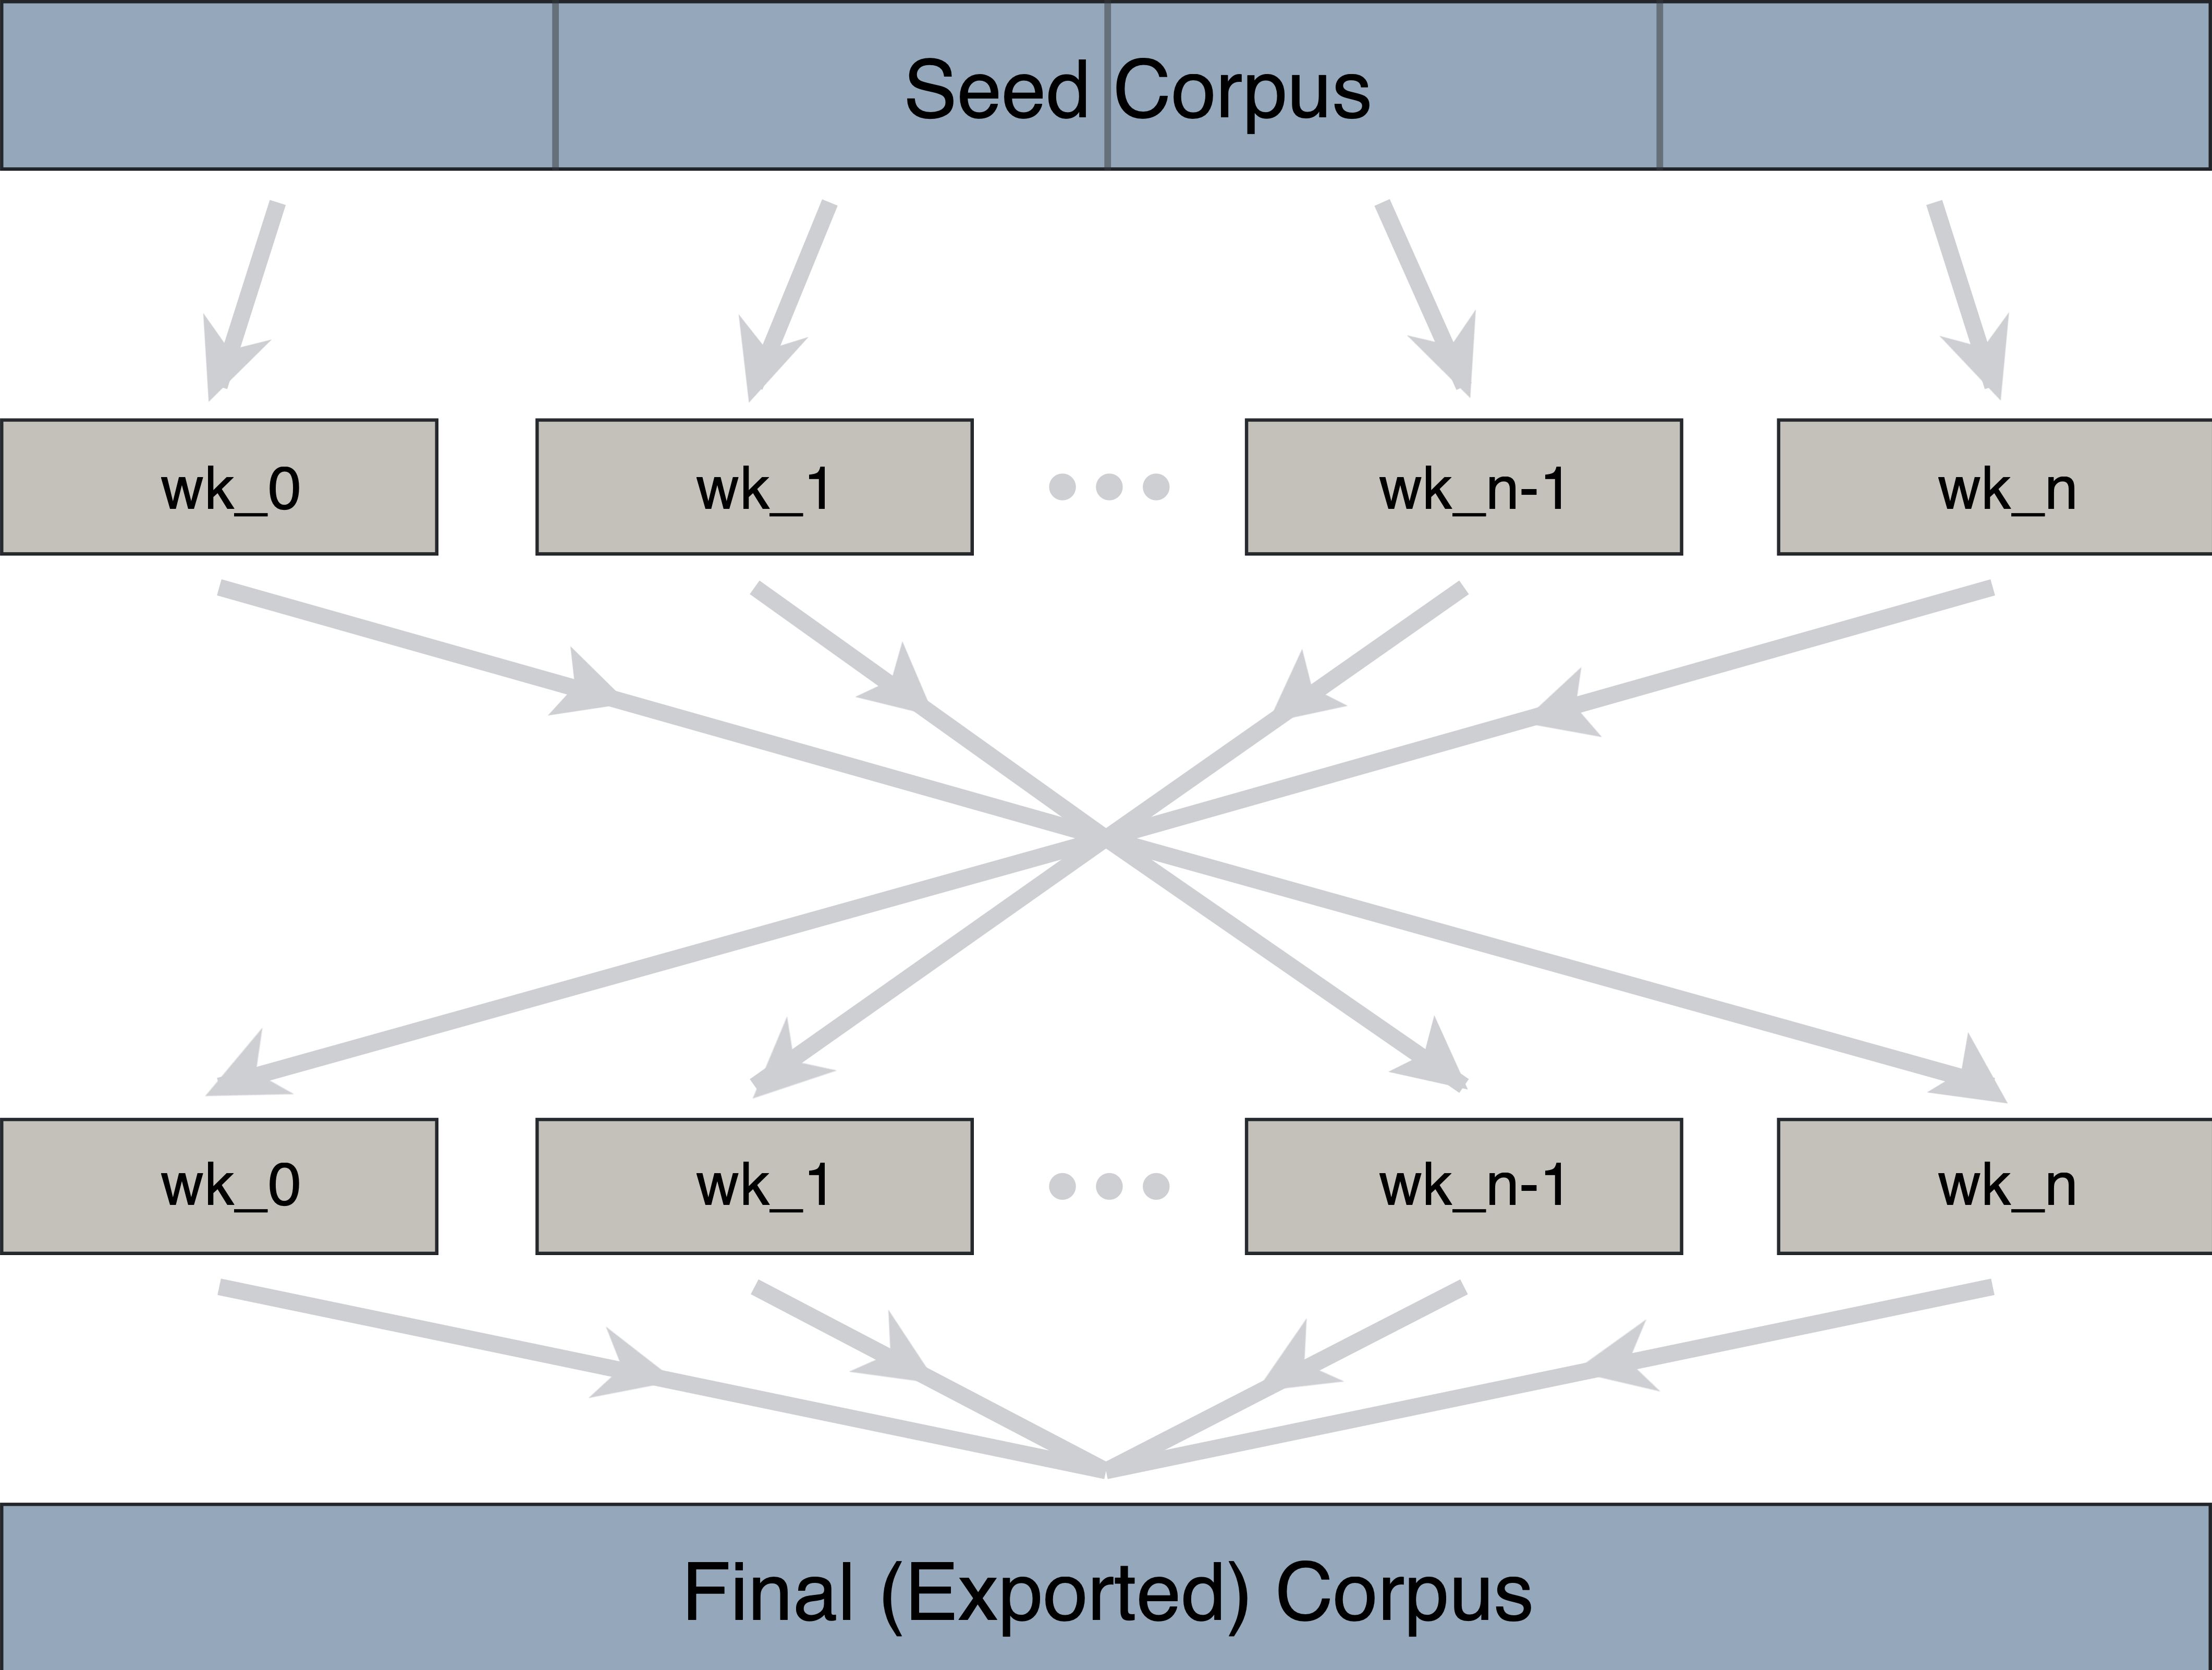
\includegraphics[width=0.45\textwidth]{./img/fuzzilli-topology}
        \caption{Scatter-Reduce-Repeat MPI fuzzing topology. Each cycle, N-equipartitions of
        the seed corpus are ingested by N fuzzing nodes, which operate for some time, then
        corpora slices concatenate and deduplicate into a single corpus.}
    \end{center}
\end{figure}\vspace{-1em}

\p{Skipping The Parser} The primary components of focus for this work are JSC's JIT compilers -- do we really need
to fuzzing the \textit{entire execution pipeline}? JS engine vulnerabilities often require a complex execution flow to trigger a
crash; fuzzing the entire pipeline ensures that we \textit{can} reach all components. Furthermore, only syntatically valid samples
make it past JSC's LLInt.

If we can assert the syntatic validity of our samples, LLInt could be skipped, effectively resulting into direct fuzzing
of \textsc{libJavaScriptCore}. Thus, we hypothesize that such an architecture would greatly improve execution speeds and results.
To test such a hypothesis Rust Foreign-Function Interfaces (FFIs) into \textsc{libJavaScriptCore} native C API were
generated using bindgen.%\cite{bindgen}.
This provided direct access to fuzz JSC's type system definitions, such as \textit{JSObject} and \textit{JSValue}

Continued exploratory testing revealed potential in this approach and merits deeping investigative experiementation.

%-----------------------------------------
\subsection{Extending Code Generation: WASM}
Added wasm as an additional (minor) target $\rightarrow$ wasm isn't
JIT'd so it's a completely different control flow, but is still a
fresh section and had potential to uncover deep crashes

\begin{table}[h]
  \begin{center}
    \begin{tabular}{c c}
        \toprule
        {Constructors} & {Static Methods} \\ 
        \midrule
        \_.Global   & \_.instantiate() \\
        \_.Module   & \_.instantiateStreaming() \\
        \_.Memory   & \_.compile() \\
        \_.Instance & \_.compileStreaming() \\
        \_.Table    &  \\ [1ex]
        \bottomrule
    \end{tabular}
    \caption{JSObject WASM contructors and static methods introduced to Fuzzilli from the \textsc{WebAssembly} namespace.}
  \end{center}
\end{table}

%-----------------------------------------
\subsection{Streamlining Triage} As exporatory testing proceeded, it became painfully obvious that crash sample automation
would be required; Fuzzilli would report a crash count of five significant figures; however, not all were valid -- futhermore,
only a relatively infintesimal portion of crashes led to a valid bug. To futher complicate triage, fuzzing was performed
on a Linux distrobution, testing against the Linux build of JSC. This build differs from the macOS flavor. 

As a result, traige automation took the form of a custom script runner, executing crash samples found on the Linux fuzzing
host against the \textit{latest} ASAN build of JSC on macOS.

%===============================================================
